\Needspace{0.42\textheight}
\subsection{结果分析}

\Needspace{4\baselineskip}
\noindent\textbf{（1）温度分布}

规定时刻和径向位置的温度见表~\ref{tab:q1-temperature}，结果保留四位小数。

\input{tables/q1_temperature}

由表~\ref{tab:q1-temperature} 可知，\textbf{药材表面先升温，中心响应滞后}，这是由于表面直接与热风换热，而中心升温依赖内部导热。$1800\,\mathrm{s}$ 时，中心与表面温度相差 $3.2102\,{}^\circ\mathrm{C}$，且均低于同期烘房温度 $41.5130\,{}^\circ\mathrm{C}$，说明预热阶段结束时仍存在内外温差。

\Needspace{4\baselineskip}
\noindent\textbf{（2）含水率分布}

相同时空位置的干基含水率见表~\ref{tab:q1-moisture}。

\input{tables/q1_moisture}

由表~\ref{tab:q1-moisture} 可知，\textbf{失水主要集中在外层}。$1800\,\mathrm{s}$ 时，表面含水率已降至 $1.5102\,\mathrm{kg/kg}$，半径 $1\,\mathrm{cm}$ 处仍接近初值。中心结果在四位小数下为 $2.5500$，表明其变化很小。

\Needspace{0.62\textheight}
\noindent\textbf{（3）传递特征}

将温度和含水率的径向分布及时间变化绘于图~\ref{fig:q1-fields}。

\begin{figure}[H]
\centering
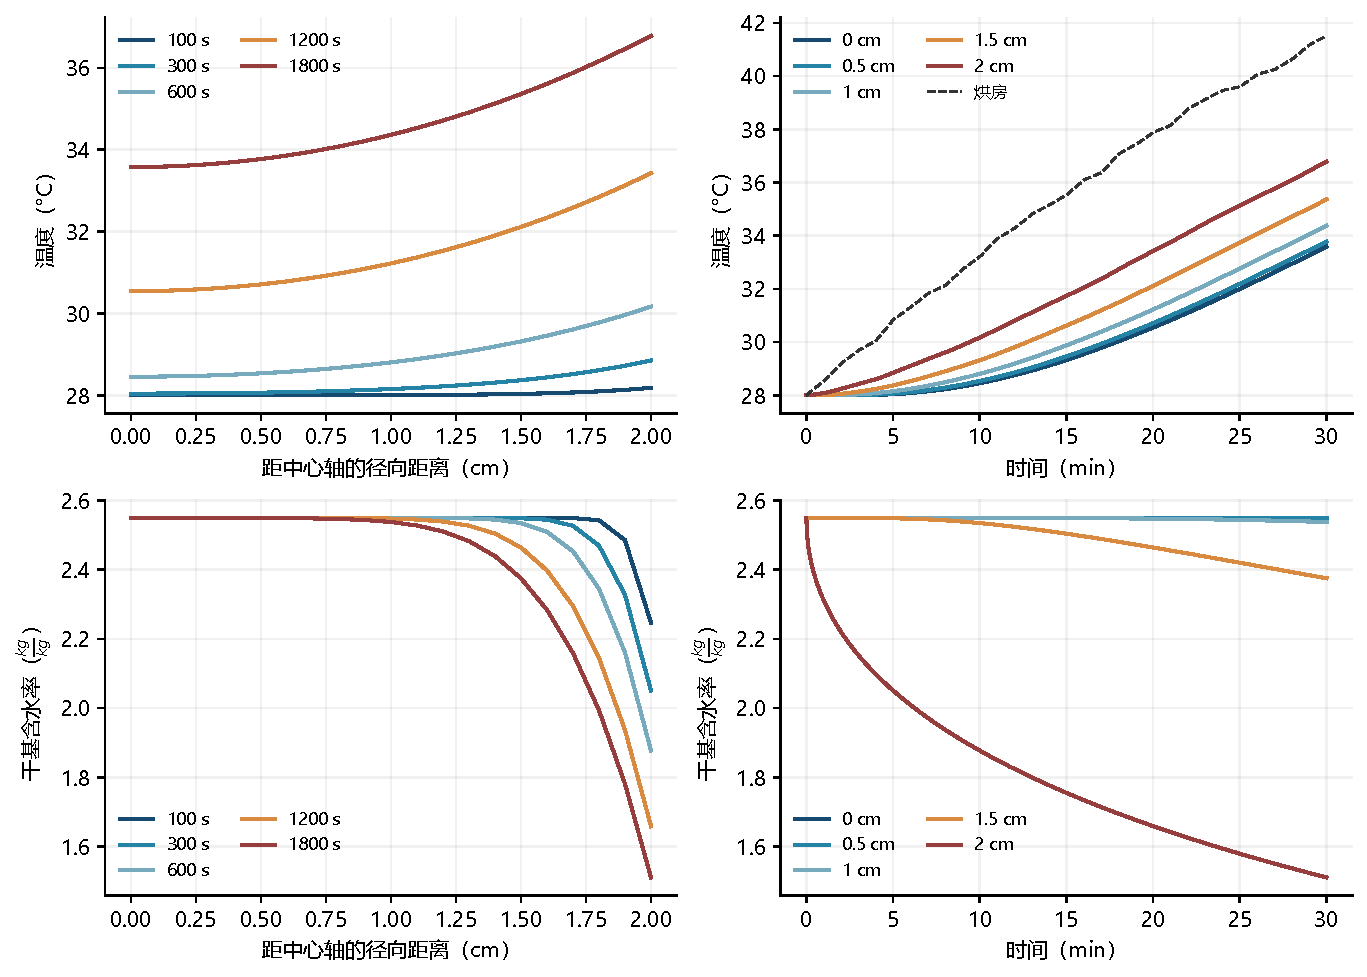
\includegraphics[width=\textwidth]{figures/q1_fields.pdf}
\caption{预热阶段温度与含水率的径向分布及时间变化}
\label{fig:q1-fields}
\end{figure}

图~\ref{fig:q1-fields} 显示，温度变化逐步传至中心，而明显失水仍局限于外层，与热扩散率高于水分扩散系数的量级关系一致。此外，$C$ 减小时 $D(C)$ 随之减小，外层干燥后水分向表面的扩散补给进一步受限。$1800\,\mathrm{s}$ 时，体积加权平均含水率由 $2.5500$ 降至 $2.2936\,\mathrm{kg/kg}$，下降 $10.0566\%$；结合径向差异可知，\textbf{此时药材尚未均匀干燥}。

本问得到的温度与含水率分布回答了预热阶段的时空变化问题。后续在此方程与数值处理框架中引入状态相关物性，可进一步描述全过程的传热传质。
